\documentclass[border=10pt]{standalone}

\usepackage{tikz}
\usepackage{tikzsymbols}
\usetikzlibrary{calc,patterns,shapes.geometric}

\def\centerarc[#1](#2)(#3:#4:#5){\draw[#1] ($(#2)+({#5*cos(#3)},{#5*sin(#3)})$) arc (#3:#4:#5);}

\begin{document}
	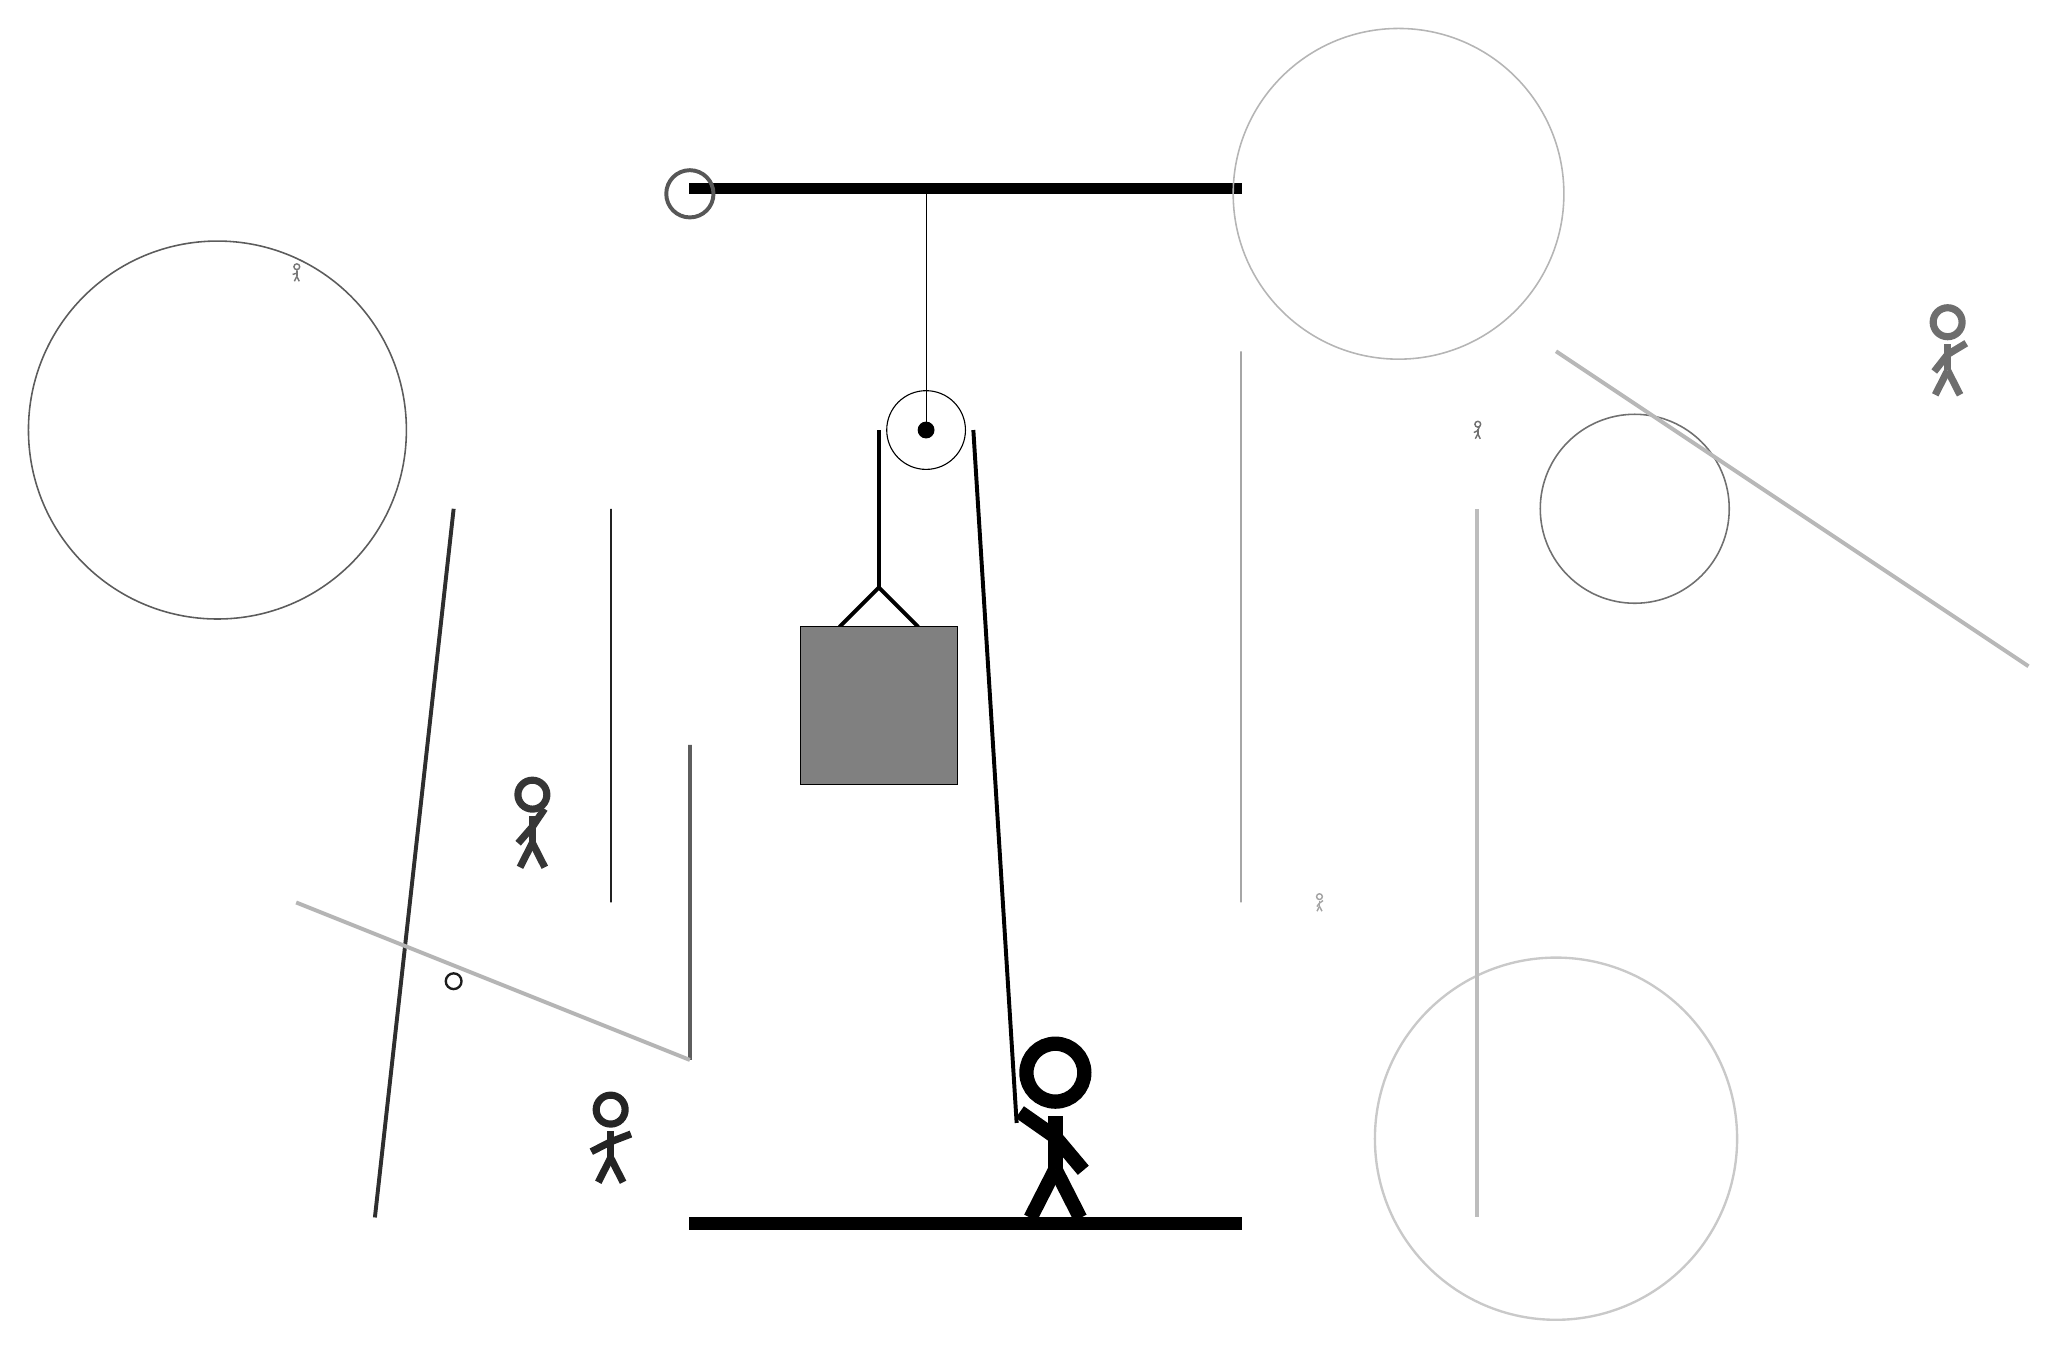
\begin{tikzpicture}
		%%%%% START %%%%%
		
		\draw[fill=black] (-2, 10) rectangle (5, 10.125);
		
		\draw[line width=0.6mm, color=black!63] (-2, 3) rectangle (-2, -1);
		
		\node[line width=0.3mm, color=black!57] at (14, 8) {\Strichmaxerl[5][52][31]};
		\draw[line width=0.5mm, color=black!82](-5, 6) -- (-6, -3);
		\draw [line width=0.2mm, color=black!56](10, 6) circle (1.2);
		\draw [line width=0.2mm, color=black!29](7, 10) circle (2.1);
		
		\draw[line width=0.5mm, color=black!29](-7, 1) -- (-2, -1);
		\draw [line width=0.3mm, color=black!21](9, -2) circle (2.3);
		\draw[line width=0.3mm, color=black!87] (-3, 6) rectangle (-3, 1);
		\draw [line width=0.3mm, color=black!89](-5, 0) circle (0.1);
		
		\draw[line width=0.5mm, color=black!28](9, 8) -- (15, 4);
		\node[line width=0.2mm, color=black!36] at (6, 1) {\Strichmaxerl[1][54][35]};
		
		\draw [line width=0.5mm, color=black!66](-2, 10) circle (0.3);
		\node[line width=0.5mm, color=black!56] at (8, 7) {\Strichmaxerl[1][25][69]};
		
		\node[line width=0.7mm, color=black!53] at (-7, 9) {\Strichmaxerl[1][17][86]};
		\draw[line width=0.2mm, color=black!35] (5, 8) rectangle (5, 1);
		\node[line width=0.2mm, color=black!79] at (-4, 2) {\Strichmaxerl[5][49][56]};
		\draw[line width=0.5mm, color=black!26](8, 6) -- (8, -3);
		\draw [line width=0.2mm, color=black!64](-8, 7) circle (2.4);
		\node[line width=0.7mm, color=black!86] at (-3, -2) {\Strichmaxerl[5][27][21]};
		
		\draw (1, 7) circle (0.5);
		\draw[fill=black] (1, 7) circle (0.1);
		\draw (1, 10) -- (1, 7);
		
		\draw[line width=0.5mm] (-0.1, 4.5) -- (0.4, 5.0) -- (0.9, 4.5);
		\draw[fill=black!50] (-0.6, 4.5) rectangle (1.4, 2.5);
		
		\draw[line width=0.5mm] (0.4, 7) -- (0.4, 5.0);
		\centerarc[line width=0.5mm](1, 7)(0:180:0.6);
		\draw[line width=0.5mm](1.6, 7) -- (2.15, -1.8);
		
		\node at (2.6, -1.9) {\Strichmaxerl[10][-35][-50]};
		
		\draw[fill=black] (-2, -3) rectangle (5, -3.15);
		
		%%%%% END %%%%%
	\end{tikzpicture}
\end{document}